% !TeX spellcheck = en_US
%% Beispiel-Präsentation mit LaTeX Beamer im KIT-Design
%% entsprechend den Gestaltungsrichtlinien vom 1. August 2020
%%
%% Siehe https://sdqweb.ipd.kit.edu/wiki/Dokumentvorlagen

%% Beispiel-Präsentation
\documentclass[en,16:9]{sdqbeamer} 

\usepackage{tikz}
\usetikzlibrary{positioning,calc,arrows}
 
 
%% Titelbild
\titleimage{banner_2020_kit}

%% Gruppenlogo
\grouplogo{} 

%% Gruppenname
\groupname{Compilerpraktikum - Abschlusspräsentation}

% Beginn der Präsentation

\title[]{Compilerpraktikum - Abschlusspräsentation}
\subtitle{Gruppe 5} 
\author[]{Achim Kriso, Marc Huisinga, Erik Kristiansen, Philipp Schaback}

\date[10.\,2.\,2022]{10. Februar 2022}

% Literatur 
 
\usepackage[citestyle=authoryear,bibstyle=numeric,hyperref,backend=biber]{biblatex}
\addbibresource{presentation.bib}
\bibhang1em

\begin{document}

%Titelseite
\KITtitleframe

\begin{frame}{Front End}
	\begin{itemize}
		\item Implemented Parser Recovery
		\item Rust-style error messages
	\end{itemize}

	\begin{figure}
		\centering
		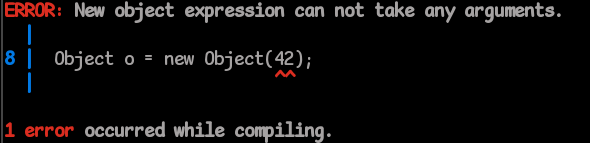
\includegraphics[draft,width=\linewidth,height=5cm]{images/error_message.png}
	\end{figure}
\end{frame}

\begin{frame}{Middle End}
	\begin{columns}
		\begin{column}{0.5\linewidth}
			\begin{itemize}
				\item Constant Folding
				\item Misc. Arithmetic Simplifications
				\item Loop invariant code motion
			\end{itemize}%
			
			\begin{figure}
				\centering
				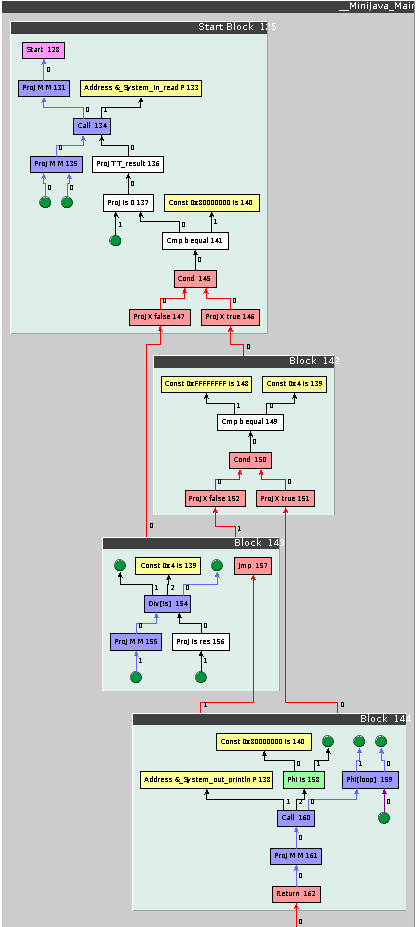
\includegraphics[draft,width=\linewidth,height=4cm]{images/optimization-before.png}
			\end{figure}
		\end{column}
		\begin{column}{0.5\linewidth}
			\begin{itemize}
				\item Common Subexpression Elimination (CSE)
				\item Function Inlining
				\item (Load/Store optimization)
			\end{itemize}
		
			\begin{figure}
				\centering
				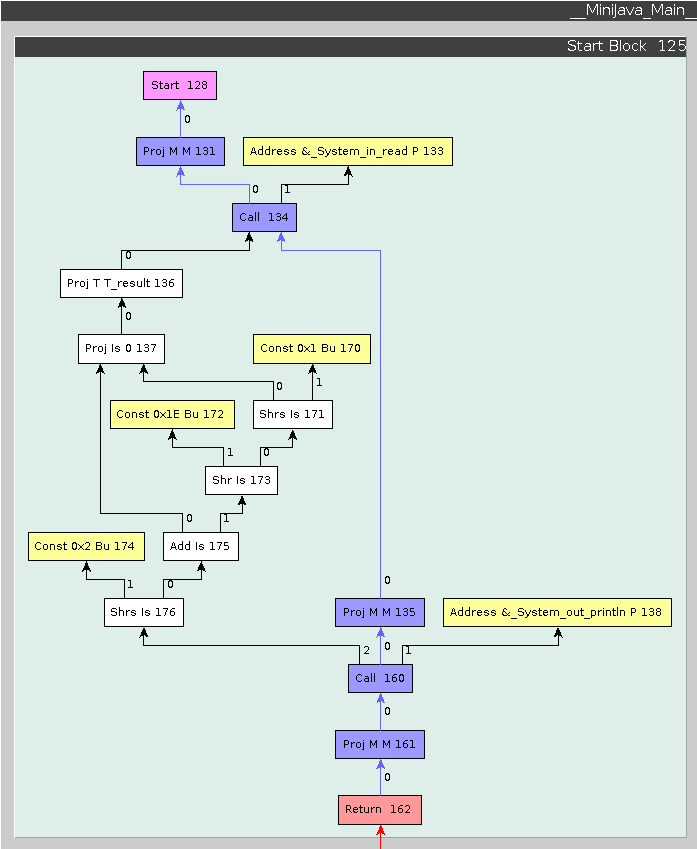
\includegraphics[draft,width=\linewidth,height=4cm]{images/optimization-after.png}
			\end{figure}
		\end{column}
	\end{columns}
\end{frame}

\begin{frame}{Back End - Overview}
	\begin{figure}
		\centering
		%\vspace{-10px}
		%\def\scale{0.7}
		\providecommand{\scale}{1}
\usetikzlibrary {positioning,arrows.meta,backgrounds,fit,positioning}
\begin{tikzpicture}[->,node distance=20mm,
	terminal/.style={
	% The shape:
	rectangle,minimum size=6mm,rounded corners=3mm,
	% The rest
	draw=black,
	font=\ttfamily},
	el/.style={
		midway,
		above,
	}]

	\node (input) [terminal] {Input};
	\node (ast) [terminal,right=of input] {AST};
	\node (firm) [terminal,right=of ast] {\textsc{Firm}};
	\node (llir) [terminal,below=of ast] {LLIR};
	\node (sir) [terminal,below=of firm] {SIR};
	\node (asm) [terminal,right=of sir] {Assembly};

\draw
	(input)	edge [el] node [] {} (ast)
	(ast)	edge [el] node [] {} (firm)
	(firm)	edge [el,out=-90,in=90] node [right] {instruction selection} (llir)
	(llir)	edge [el] node [] {scheduling} (sir)
	(sir)	edge [el,loop below] node [] {register allocation} (sir)
			edge [el] node [] {} (asm);


\begin{scope}[on background layer]
\node [fill=black!10,inner sep=20,fit=(ast) (firm)] {};
\node [fill=black!10,inner sep=26,fit=(llir) (sir)] {};
\end{scope}

% \draw [->] (input) 
% 		-- (ast) node [el] {}
% 		-- (firm) node [el] {}
% 		-- (llir) [loop,below]
% 		-- (llir) node [el,right] {instruction selection}
% 		-- (sir) node [el] {scheduling}
% 		-- (asm) node [el] {};
\end{tikzpicture}
\def\scale{1}

	\end{figure}
\end{frame}

\begin{frame}{Back End - LLIR}
	\framesubtitle{Low-Level Intermediate Representation}
	
	\begin{itemize}
		\item Graph-based
		\item Nodes represent x86 instructions
	\end{itemize}

	\begin{figure}
		\centering
		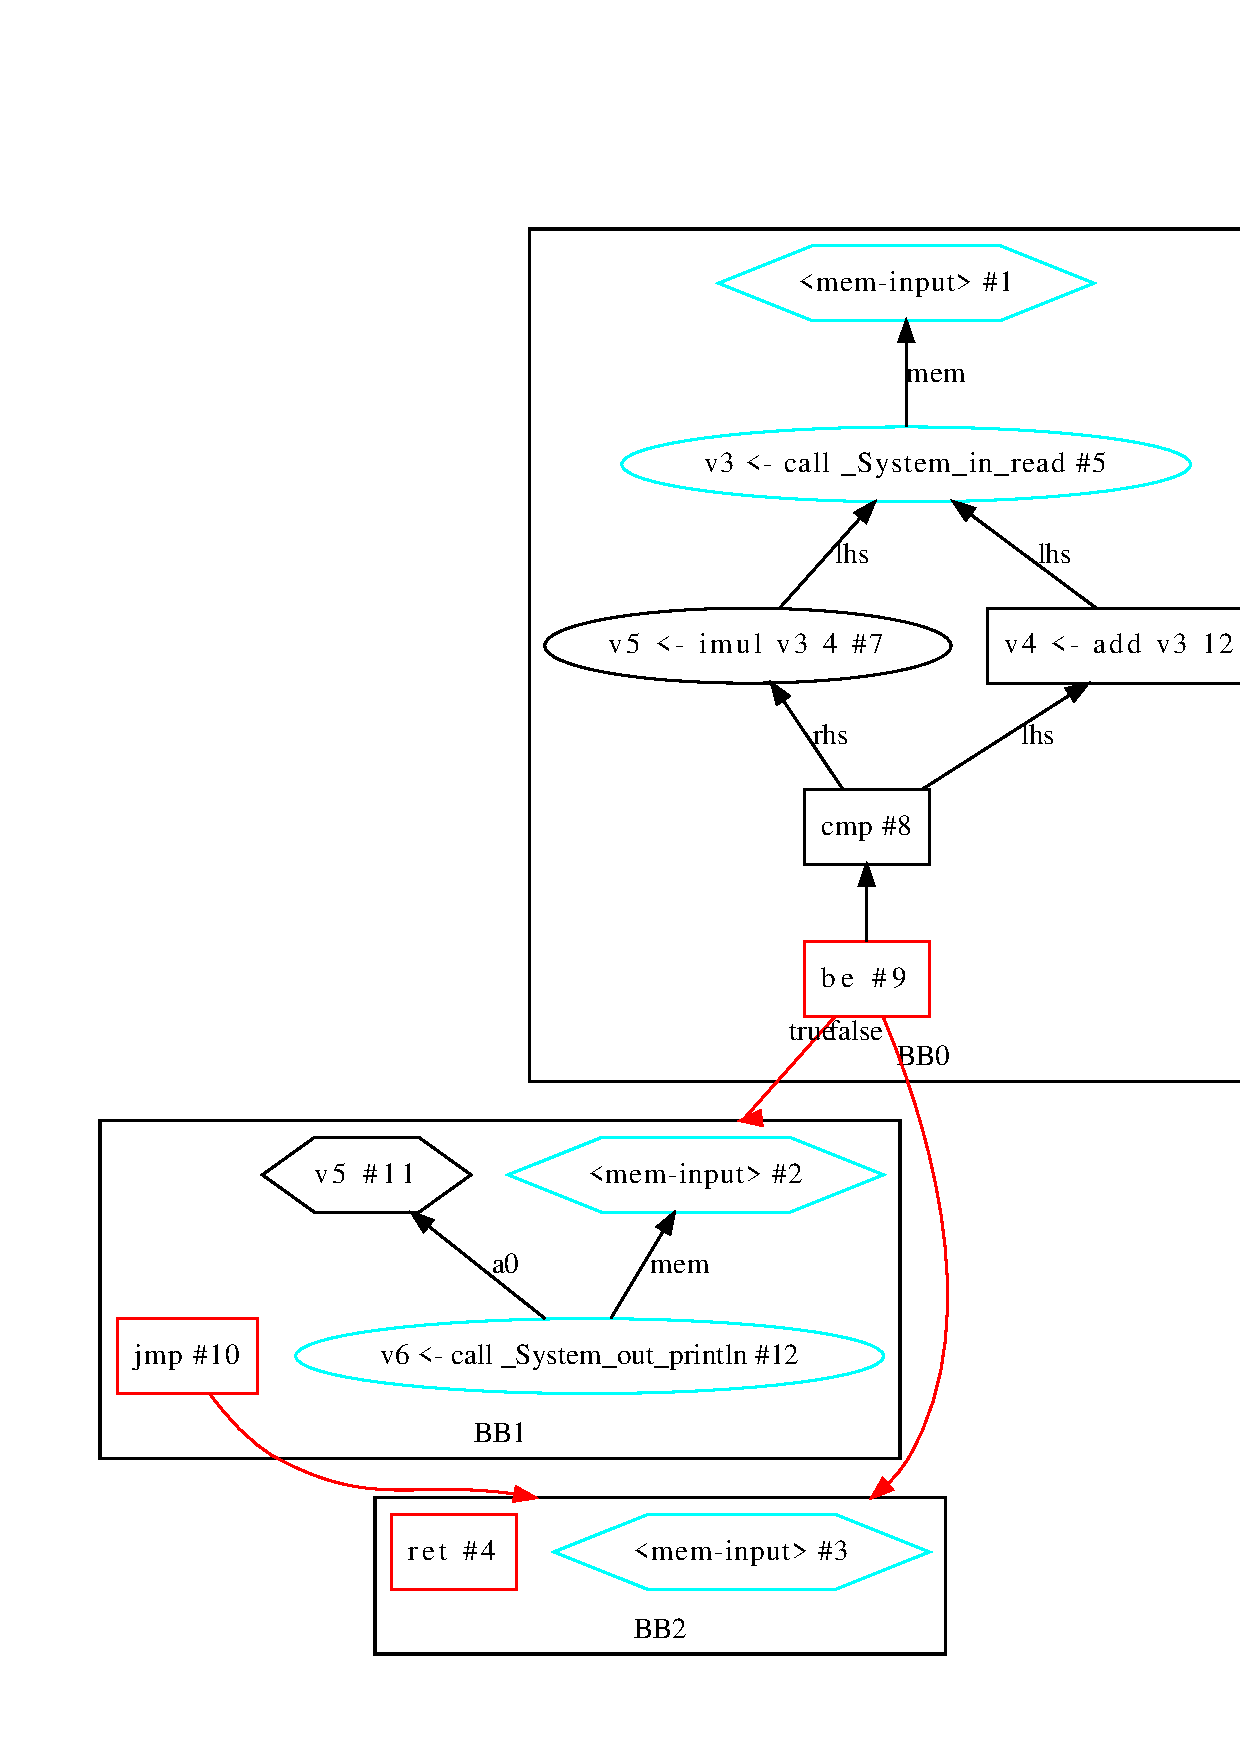
\includegraphics[draft,width=\linewidth,height=5cm]{images/llir-example.png}
	\end{figure}
\end{frame}

\begin{frame}{Back End - SIR}
	\framesubtitle{Scheduled Intermediate Representation}
	
	\begin{itemize}
		\item Includes scheduling information
		\item Modified by peephole optimizer
	\end{itemize}
	
	\begin{figure}
		\centering
		\includegraphics[draft,width=\linewidth,height=5cm]{images/sir-example.png}
	\end{figure}
	
\end{frame}

\begin{frame}{Back End - SIR}
	\framesubtitle{Scheduled Intermediate Representation}
	
	\begin{figure}
		\centering
		\includegraphics[draft,width=\linewidth,height=0.7\textheight]{images/sir-example.png}
	\end{figure}
	
\end{frame}

\appendix
\beginbackup

\begin{frame}{References}
\printbibliography
\end{frame}


\backupend

\end{document}
